\documentclass[11pt]{article}
\usepackage[sc]{mathpazo} %Like Palatino with extensive math support
\usepackage{fullpage}
\usepackage[authoryear,sectionbib,sort]{natbib}
\linespread{1.7}
\usepackage[utf8]{inputenc}
\usepackage{lineno}
\usepackage{titlesec}
\usepackage{amsfonts,amssymb,amsmath,hyperref}
\usepackage{graphicx}
\titleformat{\section}[block]{\Large\bfseries\filcenter}{\thesection}{1em}{}
\titleformat{\subsection}[block]{\Large\itshape\filcenter}{\thesubsection}{1em}{}
\titleformat{\subsubsection}[block]{\large\itshape}{\thesubsubsection}{1em}{}
\titleformat{\paragraph}[runin]{\itshape}{\theparagraph}{1em}{}[. ]\renewcommand{\refname}{Literature Cited}

%%%%%%%%%%%%%%%%%%%%%
% Line numbering
%%%%%%%%%%%%%%%%%%%%%
%
% Please use line numbering with your initial submission and
% subsequent revisions. After acceptance, please turn line numbering
% off by adding percent signs to the lines %\usepackage{lineno} and
% to %\linenumbers{} and %\modulolinenumbers[3] below.
%
% To avoid line numbering being thrown off around math environments,
% the math environments have to be wrapped using
% \begin{linenomath*} and \end{linenomath*}
%
% (Thanks to Vlastimil Krivan for pointing this out to us!)

\title{Heritable symbionts alter host life history schedules}

% This version of the LaTeX template was last updated on
% May 11, 2023.

%%%%%%%%%%%%%%%%%%%%%
% Authorship
%%%%%%%%%%%%%%%%%%%%%
% Please remove authorship information while your paper is under review,
% unless you wish to waive your anonymity under double-blind review. You
% will need to add this information back in to your final files after
% acceptance.

\author{Bell Scherick$^{1}$ \\ 
Ali M. Campbell$^{1}$ \\ 
Joshua C. Fowler$^{1}$ \\ 
Jacob Moutouama$^{1}$ \\ 
Shaun Ziegler$^{2}$ \\
Kenneth D. Whitney$^{2}$ \\
Jennifer A. Rudgers$^{2}$ \\
Tom E.X. Miller$^{1\ast}$}

\date{}

\begin{document}

\maketitle

\noindent{} 1. Department of BioSciences, Rice University, Houston, TX 77005, United States;

\noindent{} 2. Department of Biology, University of New Mexico, Albuquerque, NM 87801, United States;

\noindent{} $\ast$ Corresponding author; e-mail: tom.miller.edu.

\bigskip

\textit{Manuscript elements}: 

\bigskip

\textit{Keywords}: 

\bigskip

\textit{Manuscript type}: Article. %Or note, natural history miscellany note, comment, reply, invited symposium, featured topic, or historical perspective.

\bigskip

\noindent{\footnotesize Prepared using the suggested \LaTeX{} template for \textit{Am.\ Nat.}}

\linenumbers{}
\modulolinenumbers[3]

\newpage{}

\section*{Abstract}



\newpage{}

\section*{Introduction}
Endosymbioses between micro- and macro-organisms are widespread in the natural world and have played a key role in the evolution of life.
Many microbial symbionts are vertically transmitted from parent to offspring, such that survival and reproduction of the symbiont are tied to that of the host. 
Both theory and empirical evidence have shown that predominantly vertically reproducing endosymbionts are selected to act as mutualists in order to increase the reproduction of their host, and therefore themselves.
However, symbioses that are mutually beneficial in their net effects may still involve conflict of interest. 
The stability of host-symbiont mutualism therefore requires mechanisms that resolve conflict or benefits that are sufficiently strong to compensate for it. 

Microbial symbionts can induce diverse effects on age-specific survival and reproduction -- parameters that define the host life history. 
Such life history modifications may or may not constitute host-symbiont conflict depending on how they influence net fitness of hosts. 
For vertically-transmitted symbionts, selection may act to favor symbiont strategies that induce early host reproduction, which ensures symbiont fitness against the risk of host mortality or reproductive failure later in life.\footnote{All else equal, a perfectly and exclusively heritable symbiont should have the same ESS life history strategy as its host, but imperfect transmission or retention may favor symbionts getting out earlier.} 
For example, infection by the heritable bacterial symbiont \textit{Wolbachia} has been found to accelerate early host reproduction and modify age-specific survival rates in pharaoh ants \citep{singh2020wolbachia} and fruit flies \citep{fry2004variable}. 
Shield bugs carry heritable extra-cellular bacterial symbionts in the mid-gut that reduce the pre-ovipositional period by 10 days, on average \citep{karamipour2021removal}. 
Symbiont-driven shifts in host life history strategies toward a faster pace of life may still be consistent with host-symbiont mutualism, as long as positive effects of symbionts compensate for any costs associated with deviation from optimal host life history strategies. 
On the other hand, advantages of symbiosis may allow hosts to access higher-fitness strategies such that ``deviations'' of the life history schedule work in favor of both host and symbiont. 
Rarely are these alternative fitness implications known or tested \citep{karamipour2021removal}

Life history manipulation is best studied in arthropod-microbe symbioses, but plants also harbor a rich consortium of microbial associates with the potential to alter life history schedules. 
Fungal endophytes in the genus Epichlo\"{e} are obligate symbionts of cool-season grasses that are vertically-transmitted through host seed production; some Epichloe species also engage in horizontal transmission at the expense of host reproduction \citep{cheplick2009ecology,clay2002evolutionary}. 


In this study, we leverage a unique, long-term symbiont removal experiment, combined with statistical and demographic modeling, to evaluate how endophyte symbiosis modifies the trajectory of mortality and reproduction of host grasses. 
Taxonomically replicated across seven host-symbiont pairs, our 14-year field experiment has longitudinally tracked replicated cohorts of recruitment in grass populations that were established either symbiotically with \textit{Epichlo\"{e}} fungal endophytes (S+) or with endophytes eliminated through heat treatment (S-). 
By tracking multiple host cohorts that recruit in different years, our study is uniquely able to isolate, for the first time, age-specific effects of endophyte symbiosis from the confounding influence of background inter-annual variation. 
We combined statistical estimation of age- and symbiont-specific reproduction and mortality schedules with matrix projection models to synthesize the overall influence of symbiosis on host fitness and life history metrics. 
Specifically, we asked the following:
\begin{itemize}
	\item Are there age-specific effects of endophytes on host reproduction and mortality schedules?
	\item How do endophyte effects on reproduction and survival combine to influence host life history strategies?
	\item Are shifts in host life history consistent with overall host-symbiont mutualism?
	\item How consistent are the life history outcomes of symbiosis across host-symbiont taxonomic pairs, and can host and/or symbiont traits explain inter-specific variation?
\end{itemize}





\section*{Methods}
\subsection*{Experimental design}

\subsection*{Data collection}
Data collection methods follow that of our previous study \citep{fowler2024microbial}. 

\subsection*{Statistical modeling}
We used the long-term demographic data to fit statistical models for age- and symbiont-dependent vital rates. 
Model-fitting was done in a hierarchical Bayesian framework using Stan \citep{carpenter2017stan} and the `rstan' package \citep{rstan} in R version 4.2.3 \citep{R}. 
Hierarchical modeling allowed us to maximize inference by ``borrowing strength'' across taxonomic, temporal, and spatial dimensions of the experimental design. 
We fit models for three vital rates: age-specific survival, age-specific fertility, and recruitment. 
For all models, we ran three chains for 10,000 iterations with a thinning rate of 2. 
We used vague priors except where noted. 

For age-specific vital rates, age was modeled as a categorical factor rather than a continuous covariate; this allowed for maximally flexible age-dependence without having to assume a functional form of how vital rates varied with age. 
Due to mortality, sample sizes decreased with increasing age (Table).
For each species we pooled advanced ages with fewer than 10 observations each into a combined ``old'' age class. 
For example, if the oldest age with at least 10 observations was 5 years old, everything older than 5 was pooled as age class ``6+''.
When S+ and S- populations differed in the upper age that satisfied $n \geq 10$, we used the younger age of the two to define the ``old'' age group. 
This difference was most pronounced in \textit{Poa alsodes}, where the oldest age with $n \geq 10$ was $1yo$ for S- and $4yo$ for S+ (Table). 
Therefore, age classes for the \textit{P. alsodes} vital rate models were 0, 1, and 2+. 
All other host species had more even age representation between S+ and S- and greater representation of later ages, with ``old'' age groups reaching 4+ for \textit{E. villosus} and \textit{E. virginicus}, 5+ for \textit{P. autumnalis}, 6+ for \textit{A. perennans} and \textit{F. subverticillata}, and 7+ for \textit{P. sylvestris}. 

\subsubsection*{Age-specific survival}
The survival model included fixed effects of host species, age class, and enodphyte status and random effects associated with year-to-year and plot-to-plot variation. 
Let $y_{ijkl}$ be the survival status (1=alive, 0=dead) of individual $i$ of species $j$ in plot $k$ and year $l$.  
We modeled these data as Bernoulli-distributed with probability of survival $\hat{p}_{ijkl}$ given by:

\begin{align*}
	logit(\hat{p}_{ijkl}) = \alpha^{j}_{a[i]} + \beta^{j}_{a[i]} * e_k + \rho_k + \tau^{j}_{l}\\
	\rho_k \sim N(0,\sigma^2_{plot})\\
	\tau^{j}_{l} \sim N(0,\sigma^2_{year})\\
	\label{eq:surv_mod}
\end{align*}

Factor variable $a[i]$ is the age class of individual $i$ in year $l$ and $e_k$ is the endophyte status (1=S+, 0=S-) assigned to plot $k$, which we assume to apply equally to all individuals in plot $k$. 
Parameter $\alpha^{j}_{a}$ is the survival probability of species $j$ age class $a$ (on the logit scale) and parameter $\beta^{j}_{a}$ is the effect of endophyte symbiosis on that survival rate. 
Host species share variance parameters ($\sigma^2$) for plot ($\rho_k$) and year ($\tau^{j}_{l}$) effects. 
Year effects $\tau^{j}_{l}$ are expicitly associated with species $j$, allowing different species to experience good and bad years at different times (while sharing the same variance).
Because each plot contains only one species, plot effects $\rho_k$ are implictly associated with species $j$.
We used the weakly informative priors $\alpha^{j}_{a} \sim N(-1,5)$, indicating that plants are more likely to die than survive, on average, with one standard deviation below and above the mean corresponding to $0.24\%$ and $98\%$ survival probabilities, respectively.
These priors accommodated a wide range of potential model outcomes while pointing the algorithm in the right direction to aid convergence. 

\subsubsection*{Age-specific fertility}
The fertility model was similar in structure to the survival model except that the response variable was the count of inflorescences of individual $i$ of species $j$ in plot $k$ and year $l$. 
We modeled these counts as Negative Binomially-distributed with mean $\mu_{ijkl}$ and species-specific overdispersion $\phi_{j})$. 
$log(\mu_{ijkl})$ was given by the same linear predict as $logit(\hat{p}_{ijkl})$ in Eq. \ref{eq:surv_mod}. 
Overdispersion parameters were modeled as a Gamma-distributed species random effect $\phi_{j} \sim Gamma(\alpha^\phi,\beta^\phi)$ with cross-species mean $\frac{\alpha^\phi}{\beta^\phi}$. 
While the inflorescence counts were zero-heavy, posterior predictive checks confirmed that the negative binomial model could generate the observed frequencies of zeroes. 

\subsubsection*{Recruitment rate}
Finally, we modeled the number of recruits of species $j$ observed in plot $k$ and year $l$ as Poisson-distributed with mean $\lambda_{jkl}$. 
We defined this mean as a function of the total number of inflorescneces ($inf$) produced in plot $k$ in the previous year $l-1$, allowing for random plot and year effects as above:
\begin{align*}
	\lambda_{jkl} = r^{1}_{jk} * inf_{k,l-1} + r^{2}_{jk} * inf_{k,l-2} + 0.01\\
	r^{1}_{jk} = exp(\alpha1^{j} + \beta1^{j}*e_k + \rho_k + \tau^{j}_{l})\\
	r^{2}_{jk} = exp(\alpha2^{j} + \beta2^{j}*e_k + \rho_k + \tau^{j}_{l})\\	\rho_k \sim N(0,\sigma^2_{plot})\\
	\tau^{j}_{l} \sim N(0,\sigma^2_{year})\\
\end{align*}
Species-specific parameters $\alpha^{j}$ control the rate at which last year's inflorescences generate this year's recruitment, and parameters $\beta^{j}$ control endophyte effects on this rate. 
Note that the model is agnostic to \emph{how} endophytes effect the inflorescence-to-recruitment rate (e.g., through effects on seed number per inflorescence, seed germination rate, or seedling survival). 
The covariate $inf_{k,l}$ was calculated for each plot by summing inflorescences across all individuals, including the original plants that are otherwise not included in these analyses, since their reproduction contributed to observed recruitment. 
We assume that recruitment occurs exclusively from seed production in the preceding year, i.e., no long-lived seed bank. 
Eq. \ref{eq:recruit_mod} implies that if no inflorescences are produced in a plot, there should be no recruitment in the following year (mostly true??). 

\subsection*{Demographic modeling}

\section*{Results}

\begin{figure}
	\begin{center}
		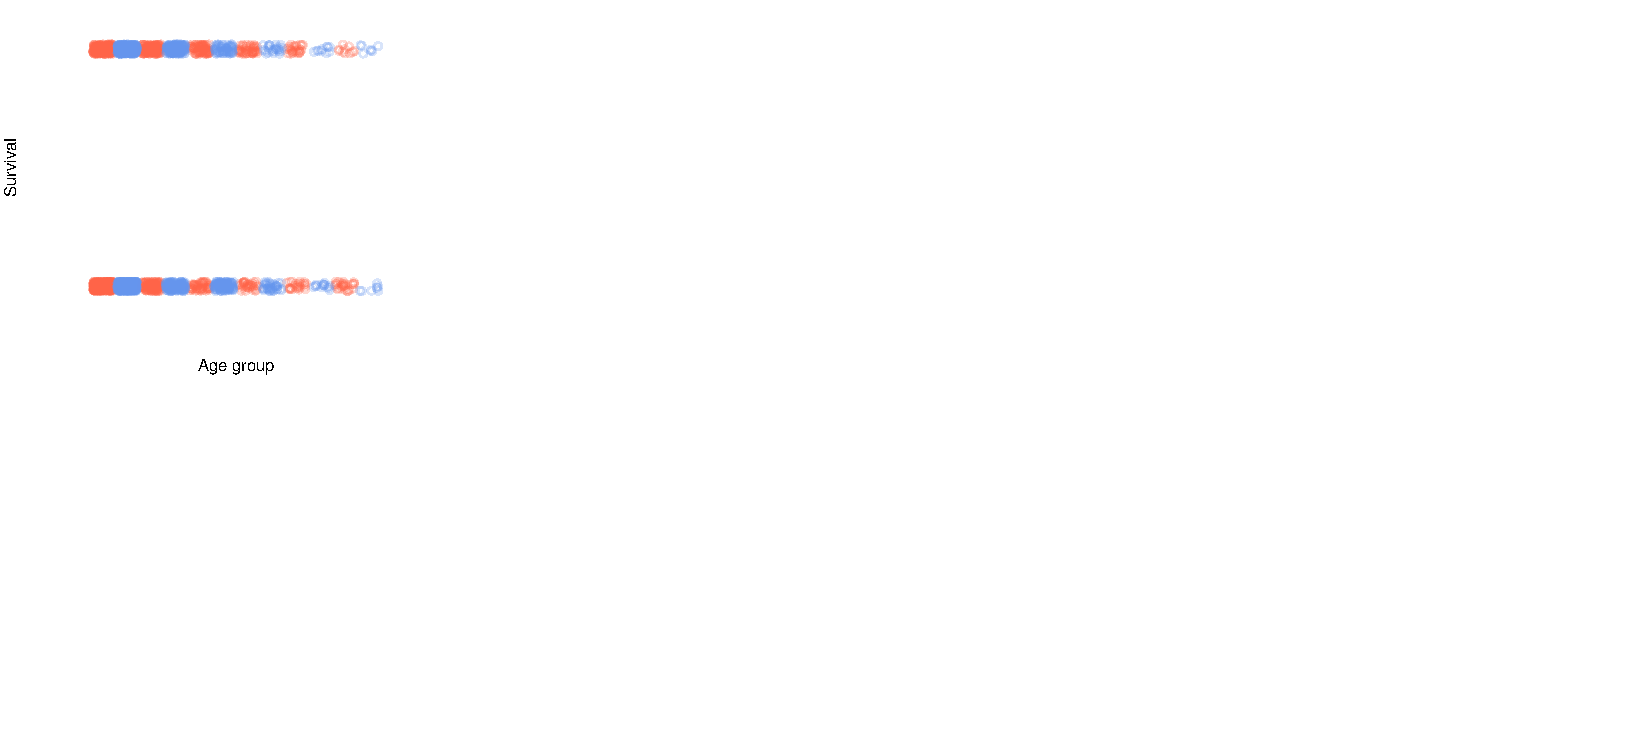
\includegraphics[width=1\linewidth]{figures/age_specific_survival}
		\caption{}
		\label{fig:age_surv}
	\end{center}
\end{figure}


\begin{figure}
	\begin{center}
		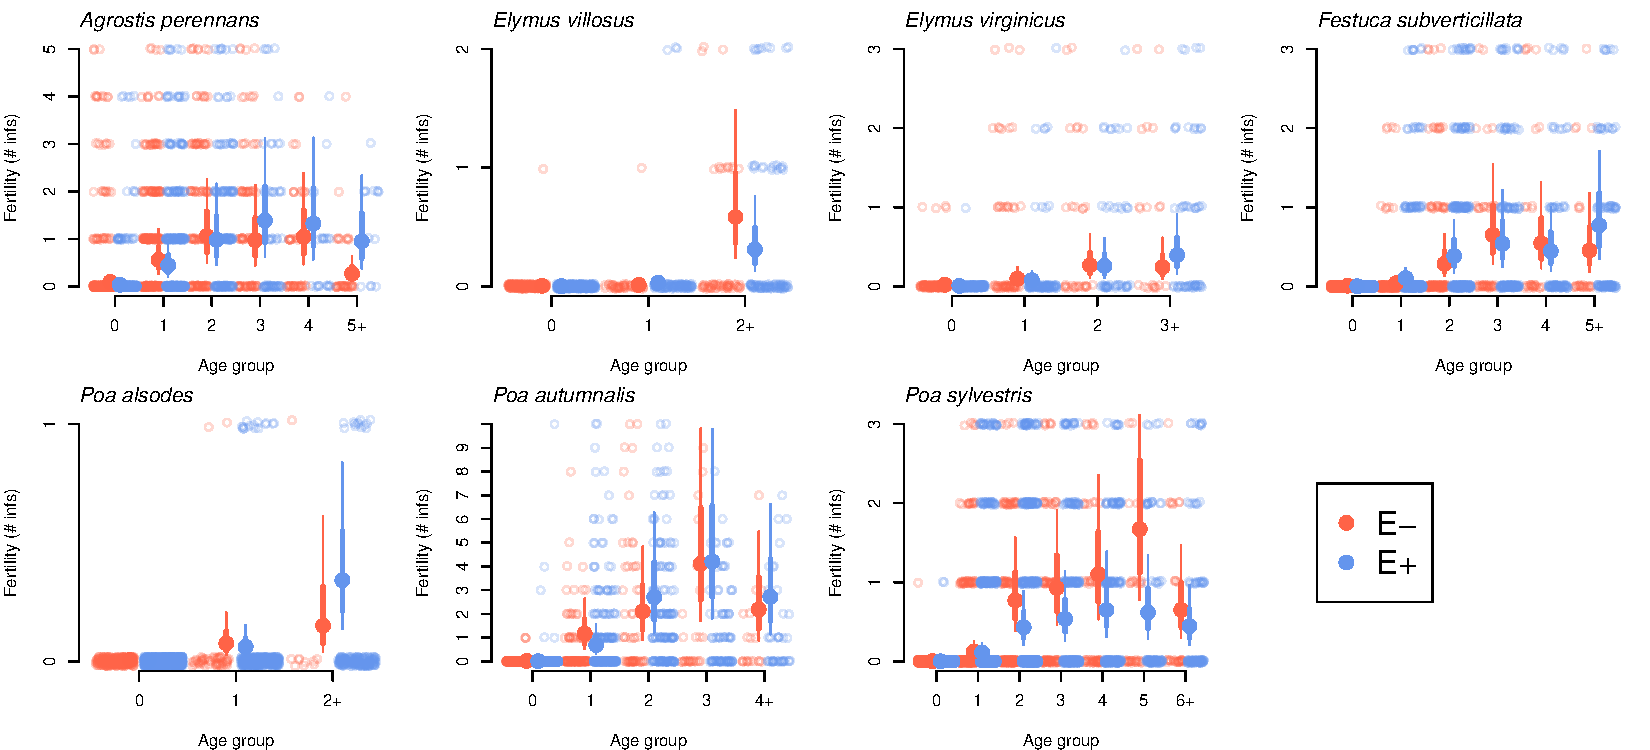
\includegraphics[width=1\linewidth]{figures/age_specific_fertility}
		\caption{}
		\label{fig:age_surv}
	\end{center}
\end{figure}

\begin{figure}
	\begin{center}
		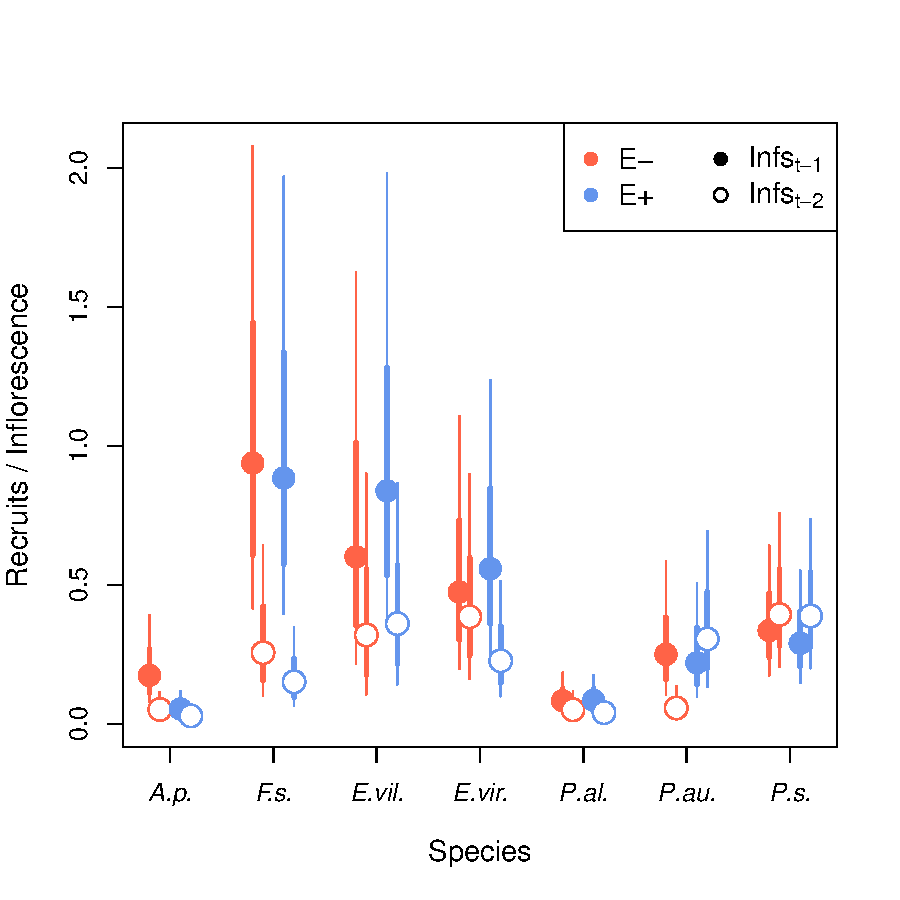
\includegraphics[width=0.75\linewidth]{figures/recruitment}
		\caption{}
		\label{fig:recruitment}
	\end{center}
\end{figure}

\section*{Discussion}

\section*{Conclusion}



%%%%%%%%%%%%%%%%%%%%%
% Acknowledgments
%%%%%%%%%%%%%%%%%%%%%
% You may wish to remove the Acknowledgments section while your paper 
% is under review (unless you wish to waive your anonymity under
% double-blind review) if the Acknowledgments reveal your identity.
% If you remove this section, you will need to add it back in to your
% final files after acceptance.

\section*{Acknowledgments}


%%%%%%%%%%%%%%%%%%%%%
% Statement of Authorship
%%%%%%%%%%%%%%%%%%%%%
% This section should also be commented out while your MS is undergoing
% double-blind review. The specifics should of course be adapted to
% your paper, but the paragraph below gives some hints of possible
% contributions.

\section*{Statement of Authorship}



\section*{Data and Code Availability}
 

\section*{Appendix A: Additional Methods and Parameters}

% In most cases, authors should typeset supplementary material in a separate,
% author-supplied PDF. For author-supplied PDFs, please consult the
% AmNat_supp_template.tex document, available from
% https://www.journals.uchicago.edu/journals/an/instruct 
%
% By contrast, the Appendix instructions below apply to cases in which
% a brief appendix is to appear in print after the main body of the article.
% That notably includes descriptions of methods, tables defining parameters,
% and other material necessary for reproducing the MS's results.
%
% Please reset counters for the appendix (thus normally figure A1, 
% figure A2, table A1, etc.).
%
% Most AmNat articles have no more than one print appendix. If your article
% has more than one, counters for each appendix should match the letter of
% that appendix. For example, tables in Appendix B should be numbered table B1, % table C2, etc. This applies to tables, equations, and figures.
%
% It's better not to use the \appendix command, because we have some
% formatting peculiarities that \appendix conflicts with.

\renewcommand{\theequation}{A\arabic{equation}}
% redefine the command that creates the equation number.
\renewcommand{\thetable}{A\arabic{table}}
\setcounter{equation}{0}  % reset counter 
\setcounter{figure}{0}
\setcounter{table}{0}

\begin{table}[ht]
	\centering
	\begin{tabular}{rrrrrrrrr}
		\hline
		Endo & Age & AGPE & ELRI & ELVI & FESU & POAL & POAU & POSY \\ 
		\hline
		0 & 0 & 678 & 258 & 125 & 809 & 253 & 816 & 2516 \\ 
		0 & 1 & 256 & 50 & 63 & 253 & 58 & 160 & 527 \\ 
		0 & 2 & 135 & 19 & 36 & 106 & 8 & 66 & 229 \\ 
		0 & 3 & 83 & 15 & 12 & 47 & 3 & 36 & 131 \\ 
		0 & 4 & 50 & 9 & 5 & 30 & 0 & 18 & 70 \\ 
		0 & 5 & 26 & 8 & 3 & 13 & 0 & 5 & 39 \\ 
		0 & 6 & 7 & 7 & 3 & 6 & 0 & 3 & 19 \\ 
		0 & 7 & 1 & 5 & 0 & 5 & 0 & 2 & 9 \\ 
		0 & 8 & 1 & 4 & 0 & 2 & 0 & 1 & 4 \\ 
		0 & 9 & 1 & 0 & 0 & 0 & 0 & 0 & 3 \\ 
		0 & 10 & 0 & 0 & 0 & 0 & 0 & 0 & 1 \\ 
		0 & 11 & 0 & 0 & 0 & 0 & 0 & 0 & 1 \\ 
		1 & 0 & 770 & 385 & 273 & 1750 & 1135 & 1775 & 5473 \\ 
		1 & 1 & 341 & 108 & 97 & 515 & 392 & 389 & 1802 \\ 
		1 & 2 & 184 & 47 & 48 & 264 & 123 & 187 & 744 \\ 
		1 & 3 & 66 & 29 & 27 & 165 & 76 & 99 & 339 \\ 
		1 & 4 & 24 & 12 & 15 & 99 & 31 & 45 & 214 \\ 
		1 & 5 & 10 & 8 & 9 & 61 & 5 & 21 & 112 \\ 
		1 & 6 & 5 & 5 & 5 & 28 & 0 & 3 & 57 \\ 
		1 & 7 & 0 & 3 & 2 & 17 & 0 & 0 & 33 \\ 
		1 & 8 & 0 & 3 & 1 & 9 & 0 & 0 & 17 \\ 
		1 & 9 & 0 & 1 & 0 & 3 & 0 & 0 & 4 \\ 
		1 & 10 & 0 & 1 & 0 & 3 & 0 & 0 & 2 \\ 
		1 & 11 & 0 & 1 & 0 & 2 & 0 & 0 & 2 \\ 
		1 & 12 & 0 & 1 & 0 & 0 & 0 & 0 & 0 \\ 
		1 & 13 & 0 & 1 & 0 & 0 & 0 & 0 & 0 \\ 
		1 & 14 & 0 & 1 & 0 & 0 & 0 & 0 & 0 \\ 
		\hline
	\end{tabular}
\caption{Sample sizes (number of individuals) for each endophyte status (Endo), age (years), and host species.}
\label{tab:age_n}
\end{table}

%%%%%%%%%%%%%%%%%%%%%
% Bibliography
%%%%%%%%%%%%%%%%%%%%%
\bibliographystyle{apalike}
\bibliography{endo-life-history}


\end{document}
